\documentclass[12pt,a4paper,oneside]{report}

\usepackage{amsmath,amssymb}
\usepackage{graphicx}
\usepackage{booktabs,array}
\usepackage{url}
\usepackage{hyperref}

\graphicspath{{../paper/figures/}{../paper/figures/final_evaluation/}}
\hypersetup{colorlinks=true,linkcolor=black,citecolor=blue,urlcolor=blue,
  pdftitle={MOSAIC: Matched-Observation Study of Architecture-Informed Control for Hybrid QKD Routing},
  pdfauthor={Khyati Sharma},
  pdfsubject={Internship project report on hybrid QKD routing}}
\linespread{1.12}
\setlength{\textwidth}{6.27in}
\setlength{\textheight}{9.1in}
\setlength{\oddsidemargin}{0in}
\setlength{\evensidemargin}{0in}
\setlength{\topmargin}{-0.25in}
\setlength{\headheight}{14pt}
\setlength{\headsep}{0.25in}
\setlength{\parindent}{1.5em}
\setlength{\parskip}{0.25em}
\setcounter{secnumdepth}{3}
\setcounter{tocdepth}{2}
\renewcommand{\bibname}{References}

\begin{document}

\begin{titlepage}
\centering
\vspace*{1.2cm}
{\Large\bfseries MOSAIC: Matched-Observation Study of Architecture-Informed Control for Hybrid QKD Routing\par}
\vspace{1.8cm}
{\large Internship Project Report\par}
\vspace{1.0cm}
{\large submitted by\par}
\vspace{0.35cm}
{\Large\bfseries Khyati Sharma\par}
{\large Indira Gandhi Delhi Technical University for Women\\
Kashmere Gate, New Delhi -- 110006\par}
\vspace{1.1cm}
{\large under the guidance of\par}
\vspace{0.35cm}
{\Large\bfseries Dr.\ Neel Kanth Kundu\par}
\vfill
{\large Quantum Communication and Information Processing Lab\\
Centre for Applied Research in Electronics\\
Indian Institute of Technology Delhi\par}
\vspace{0.6cm}
{\large November 2026\par}
\end{titlepage}

\pagenumbering{roman}
\chapter*{Acknowledgements}
\addcontentsline{toc}{chapter}{Acknowledgements}
I would like to express my sincere gratitude to my supervisor, Dr.\ Neel Kanth Kundu, for his guidance and support throughout this project. I am thankful to the members of the Quantum Communication and Information Processing Lab for their discussions and for the research environment in which this work developed. I also thank my family for their encouragement during the project.

\chapter*{Abstract}
\addcontentsline{toc}{chapter}{Abstract}
Quantum key distribution (QKD) networks use trusted relays to extend key delivery beyond a single optical link. Routing in a hybrid fiber and free-space optical (FSO) network must account for changing link quality, security constraints, and stored key resources. This report presents a simulator-based study of constrained next-hop routing and a matched comparison between graph neural network proximal policy optimization (GNN-PPO) and a long short-term memory policy (LSTM-PPO).

Both policies share the same candidate-edge features, actor--critic decision head, PPO training budget, physical-feasibility mask, and held-out scenarios. Five independently trained checkpoints per architecture are evaluated on 540 paired episodes. LSTM-PPO completes 403 routes (74.6\%), while GNN-PPO completes 249 (46.1\%). The paired difference is 28.5 percentage points, with a nested 95\% interval of 20.6--37.2 percentage points. LSTM-PPO also has fewer successful-route hops on average and lower measured actor-call latency in the reported setup.

The result applies to the implemented encoders, topology, simulator, training procedure, and scenario matrix. In particular, the LSTM reads node features in a fixed topology order and resets its state at each decision. The modeled links, key-pool dynamics, and route geometry are not calibrated field measurements; the normalized rate is not delivered secret-key throughput. The report documents the problem, simulator, learning methods, evaluation, results, and limitations without treating the experiment as a security proof or deployment assessment.

\addcontentsline{toc}{chapter}{Contents}
\tableofcontents
\clearpage
\addcontentsline{toc}{chapter}{List of Figures}
\listoffigures
\clearpage
\addcontentsline{toc}{chapter}{List of Tables}
\listoftables
\clearpage
\pagenumbering{arabic}

\chapter{Introduction}

\section{Background and Motivation}
Quantum key distribution derives its security from quantum-mechanical properties rather than from the assumed difficulty of a classical computational problem \cite{bennett1984,scarani2009}. A direct optical link has a limited range because photon loss reduces the usable key rate as distance increases. Trusted-node networks extend service by establishing keys on adjacent links and relaying key material through intermediate nodes \cite{munro2015,ituY3800,ituY3803}. The path therefore determines not only the distance travelled, but also which link states and stored key resources are required.

Hybrid networks combine fiber links with free-space optical links. Fiber is suitable for stable corridors, while FSO links can provide alternate paths where a fiber route is unavailable or where a candidate bypass is useful. FSO quality depends on atmospheric attenuation, turbulence, pointing, and availability. These effects change across scenarios and can alter which neighboring link is feasible. Routing must therefore respond to physical and resource state rather than rely only on a fixed geometric cost.

\section{Problem Statement}
The project studies sequential next-hop selection in a modeled trusted-node QKD network. At each decision, a controller observes the current network and route context, then selects a feasible adjacent node. A shared physical-feasibility rule removes candidates that violate the link QBER or projected segment-error thresholds, or that have no positive normalized rate proxy. The learning policy ranks the remaining candidates.

The central research question is whether graph message passing improves this decision over a matched LSTM-PPO node-sequence encoder. The comparison holds the action interface and downstream PPO decision path fixed while changing the encoder. It evaluates one route per episode. It does not model traffic-level request blocking, simultaneous multi-demand service, or wavelength and time-slot assignment.

\section{Objectives and Contributions}
The objectives of this work are:
\begin{enumerate}
  \item to describe a hybrid fiber/FSO simulator in which scenario-dependent link and key-pool state enter the routing observation;
  \item to compare the graph-message-passing and ordered-node LSTM encoders under matched training budgets, action masks, and held-out scenarios;
  \item to report route completion alongside conditional route length, training-seed variation, inference cost, and reward-component diagnostics; and
  \item to document the model assumptions and delimit what the simulator results can support.
\end{enumerate}

The primary contribution is a controlled comparison of two implemented policy architectures in this simulator. The main result favors LSTM-PPO on the frozen held-out scenario matrix. It does not establish that LSTM architectures are generally better than GNN architectures, nor does it demonstrate field performance.

\section{Report Organization}
Chapter~2 reviews the QKD, routing, and learning concepts relevant to the study. Chapter~3 defines the routing problem and its simulator quantities. Chapter~4 describes the topology, encoders, PPO procedure, and matched experimental protocol. Chapter~5 reports the held-out results and diagnostics. Chapter~6 discusses their interpretation and limits. Chapter~7 summarizes the answer and identifies follow-up studies.

\chapter{Literature Survey}

\section{QKD Links and Trusted-Node Networks}
The BB84 protocol uses non-orthogonal states to detect disturbance and establish shared key material \cite{bennett1984}. Practical systems use weak coherent pulses and decoy-state methods to estimate single-photon contributions \cite{hwang2003,lo2005}. Security analyses must account for finite statistics, error-correction leakage, and security parameters; asymptotic rate expressions alone do not certify a finite block \cite{gllp2004,tomamichel2012,lim2014}.

Trusted-node networks extend QKD service by establishing keys between adjacent nodes and relaying material through trusted intermediate devices \cite{munro2015,ituY3803}. Link-level key generation, key-store state, and network-level routing are coupled: an end-to-end service can be limited by a weak link or by insufficient stored key material. Recent work has examined route selection and resource management in meshed networks \cite{johann2024}.

This project uses a normalized simulator rate proxy to provide a state variable for routing. It does not calculate delivered secret-key throughput and does not claim a composable security bound. Protocol-specific finite-key analysis for simplified trusted-node chains is a separate technical problem \cite{krawec2024}.

\section{Hybrid Optical Channels}
Fiber attenuation and device parameters influence link transmission, detection, and QBER. FSO channels introduce additional atmospheric and geometric effects. Engineering recommendations for terrestrial FSO links identify local meteorological and path information as important inputs to credible design \cite{ituP1814,krzic2023}. The present simulator varies conditions by season and time of day, but the distributions are scenario assumptions rather than fits to local weather traces.

\section{Routing and Resource Management}
Classical shortest-path algorithms provide reproducible solutions for fixed edge costs \cite{dijkstra1959}. A static path cost does not by itself capture changing link availability, route-history constraints, or key-pool state. QKD networking studies have considered key-store state, request-level route selection, and joint routing/resource assignment \cite{sharma2023,johann2024}. Their decision settings include traffic and resource-allocation choices that are outside this single-route experiment.

\section{Reinforcement Learning and Graph Policies}
Sequential decision problems are commonly represented by a Markov decision process (MDP), with a state, action set, transition rule, reward, and discount factor \cite{bellman1957,sutton2018}. PPO uses a clipped policy-gradient objective, and generalized advantage estimation is a standard method for estimating advantages \cite{schulman2017,schulman2016gae}. Graph neural networks aggregate information through graph neighborhoods \cite{kipf2017,hamilton2017,velickovic2018}. An LSTM processes an ordered sequence and can combine information across sequence positions \cite{hochreiter1997}.

Neither representation is universally preferable. A GNN receives graph structure through message passing. An LSTM sequence encoder depends on the ordering of rows and can mix features according to sequence position. The comparison in this report is consequently an empirical comparison between two specific implementations under a shared decision interface.

\section{Research Gap and Scope}
Prior work motivates QKD resource-aware routing, graph learning, and sequential policies. The study here isolates the encoder comparison in a hybrid-channel simulator with an explicit feasibility mask and paired held-out scenarios. Its results are narrower than a general comparison with classical algorithms: a resource-aware classical baseline has not been evaluated under the exact matched dynamic environment used here. This limitation is retained in the analysis rather than inferred away from a comparison between two learned policies.

\chapter{Problem Formulation}

\section{Network and Episode Model}
Let the modeled network at time $t$ be $G_t=(V,E,X_t)$, where $V$ is the set of modeled nodes, $E$ is the set of links, and $X_t$ stores scenario-dependent link and normalized key-pool values. An episode specifies a source, a destination, an environment condition, and random draws associated with that scenario. A route is built by selecting adjacent nodes until it reaches the destination, terminates under a modeled failure condition, or reaches the episode step limit.

The environment state includes the current and destination nodes, link conditions, route history, accumulated error state, key-pool state, and time. The policy observation exposes the selected node and edge features but does not expose future turbulence or outage draws as a forecast. This is a simulator-level state representation, not an operational network-control interface.

\section{State, Observation, and Action}
Each node has five features: city indicator, full trusted-node indicator, simplified trusted-node indicator, destination-relative distance, and normalized degree. Each candidate edge has nine features: QBER, normalized rate proxy, FSO indicator, normalized distance, projected chain error, normalized key-pool state, link-type switch, visited-node flag, and destination-distance progress. Message-passing edges use QBER, normalized rate proxy, FSO indicator, and normalized distance. The feature inventory is summarized in Table~\ref{tab:observations}.

\begin{table}[htbp]
\centering
\caption{Observation features used by the evaluated policies}
\label{tab:observations}
\begin{tabular}{@{}p{1.3in}p{4.8in}@{}}
\toprule
Feature group & Components \\
\midrule
Node (5) & City; full-TN; STN; destination-relative distance; normalized degree. \\
Candidate edge (9) & QBER; normalized rate proxy; FSO type; normalized distance; projected chain error; normalized key-pool state; link-type switch; visited-node flag; destination-distance progress. \\
Message-passing edge (4) & QBER; normalized rate proxy; FSO type; normalized distance. \\
\bottomrule
\end{tabular}
\end{table}

At the current node $v_t$, the raw candidate set consists of its adjacent nodes $\mathcal{N}(v_t)$. A feasibility indicator $m_{t,u}$ is one when the candidate edge has QBER below the threshold, a positive normalized rate proxy, and a projected segment error below the threshold. The action set is therefore
\begin{equation}
\mathcal{A}_{\mathrm{feasible}}(s_t)
=\{u\in\mathcal{N}(v_t):m_{t,u}=1\},\qquad Q_{\max}=0.11.
\label{eq:feasible}
\end{equation}
When this set is empty, the evaluator records a no-valid-action failure. Invalid actions and environment fallbacks are tracked separately.

\section{Cumulative Segment Error}
Within an untrusted segment, the simulator combines independent hop-error probabilities as a cumulative parity error. If the QBERs in that segment are $Q_1,\ldots,Q_k$, then
\begin{equation}
Q_{\mathrm{chain},k}
=\frac{1-\prod_{i=1}^{k}(1-2Q_i)}{2},
\qquad Q_{\mathrm{chain},0}=0.
\label{eq:chain}
\end{equation}
The accumulator resets on arrival at a full trusted node. The candidate feasibility mask uses the projected segment error after adding the candidate edge and requires it to remain below $Q_{\max}$.

\section{Link-Rate Proxy}
The default modeled rate is an asymptotic normalized proxy,
\begin{equation}
r_{\mathrm{proxy}}=p_{\mathrm{det}}\left[1-2h_2(Q)\right],
\qquad h_2(Q)=-Q\log_2Q-(1-Q)\log_2(1-Q),
\label{eq:proxy}
\end{equation}
where $p_{\mathrm{det}}$ is modeled detection probability, $Q$ is modeled QBER, and $h_2$ is binary entropy. The proxy is used for feasibility and reward shaping. It is not calibrated or reported as an experimentally measured key rate. An optional decoy-state finite-key mode is an engineering estimate and is not a composable proof.

\section{Reward and Learning Objective}
The reward combines progress, QBER margin, rate proxy, key-pool state, link costs, and terminal terms. For the archived defence profile, its implemented structure is
\begin{align}
r_t={}&w_pR_{p,t}+w_qR_{q,t}+w_rR_{r,t}
+w_k\left(R_{k,t}^{\mathrm{level}}+R_{k,t}^{\mathrm{delta}}\right) \nonumber\\
&-C_{\ell,t}-C_{e,t}-C_{c,t}
+C_{\mathrm{step},t}+C_{\mathrm{revisit},t}+C_{\mathrm{switch},t}\nonumber\\
&+C_{\mathrm{backtrack},t}+C_{\mathrm{arrival},t}
+C_{\mathrm{security},t}+C_{\mathrm{depletion},t}.
\label{eq:reward}
\end{align}
Progress, QBER-margin, rate, and pool terms are signed by destination-distance progress; link costs and terminal penalties are applied as implemented. Table~\ref{tab:reward} lists the weights and fixed values documented for this reward profile.

\begin{table}[htbp]
\centering
\caption{Documented reward terms for the defence profile}
\label{tab:reward}
\small
\begin{tabular}{@{}p{1.3in}p{0.9in}p{3.6in}@{}}
\toprule
Term & Weight/value & Contribution \\
\midrule
Progress & 0.2 & Destination-distance reduction, normalized by maximum edge distance. \\
QBER margin & 0.8 & Feasible projected-chain margin, signed by progress. \\
Rate proxy & 1.2 & Distance-prorated normalized link-rate utility, signed by progress. \\
Pool level/change & 0.4 each & Current normalized pool state and its change, signed by progress. \\
Latency/energy & 0.4 each & Distance-based costs with configured normalization. \\
Congestion & 0.5 & Degree cost above two incident choices at departure. \\
Step/revisit & $-0.05/-0.6$ & Fixed step and revisit costs. \\
Switch/backtrack & $-0.2/-0.5$ & Link-type switch and non-progress costs. \\
Arrival & $+4.0$ & Destination terminal bonus. \\
Security/depletion & $-30/-60$ & Terminal penalties for chain-error breach and pool depletion. \\
\bottomrule
\end{tabular}
\end{table}

The training objective is expected discounted return,
\begin{equation}
J(\theta)=\mathbb{E}_{\pi_\theta}\left[\sum_{t=0}^{T}\gamma^t r_t\right],
\label{eq:objective}
\end{equation}
subject to the feasible-action constraint in (\ref{eq:feasible}). Reward is a training signal; route completion and other separately defined evaluation metrics determine the reported comparison.

\chapter{Methodology and Implementation}

\section{Simulator Overview}
The simulator joins a topology, link models, scenario process, route environment, and policy evaluator. At each step, the environment updates the relevant link states, builds graph and candidate-edge features, applies the feasibility mask, records the selected hop, and updates route and key-pool state. Figure~\ref{fig:pipeline} summarizes the physical-to-decision flow.

\begin{figure}[htbp]
\centering
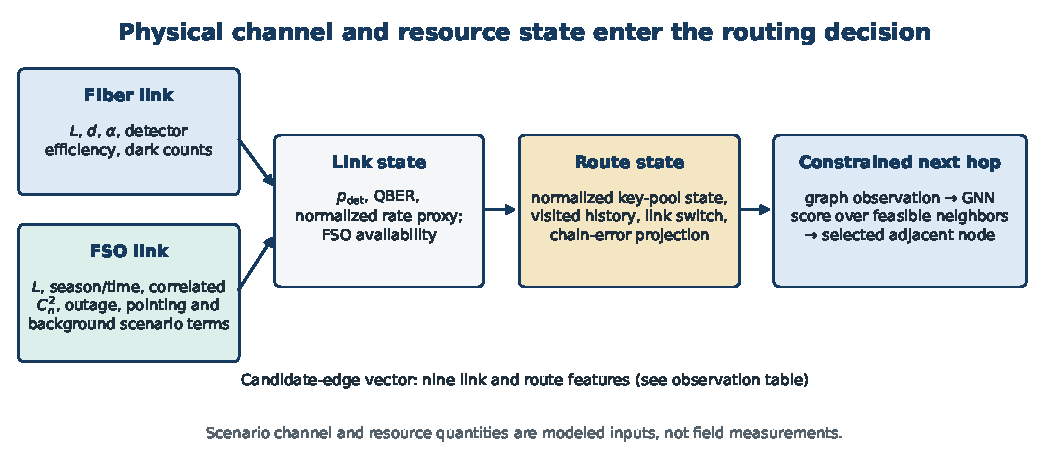
\includegraphics[width=0.95\linewidth]{physical_state_pipeline.pdf}
\caption{Physical-channel and normalized-resource state flow into feasibility-masked next-hop selection. All channel and resource values shown are simulator inputs or derived simulator quantities.}
\label{fig:pipeline}
\end{figure}

\section{Topology and Corridor Data}
The evaluated topology contains seven city hubs: Delhi, Jaipur, Mumbai, Bangalore, Hyderabad, Kolkata, and Chennai. It contains 2,370 modeled nodes and 2,653 links, comprising 273 fiber links and 2,380 candidate FSO links. OpenStreetMap driving routes provide a corridor geometry for modeled fiber paths. They are planning proxies, not verified deployed fiber routes. FSO line of sight and terrain clearance have not been surveyed. Figure~\ref{fig:topology} shows the topology and example endpoints.

\begin{figure}[htbp]
\centering
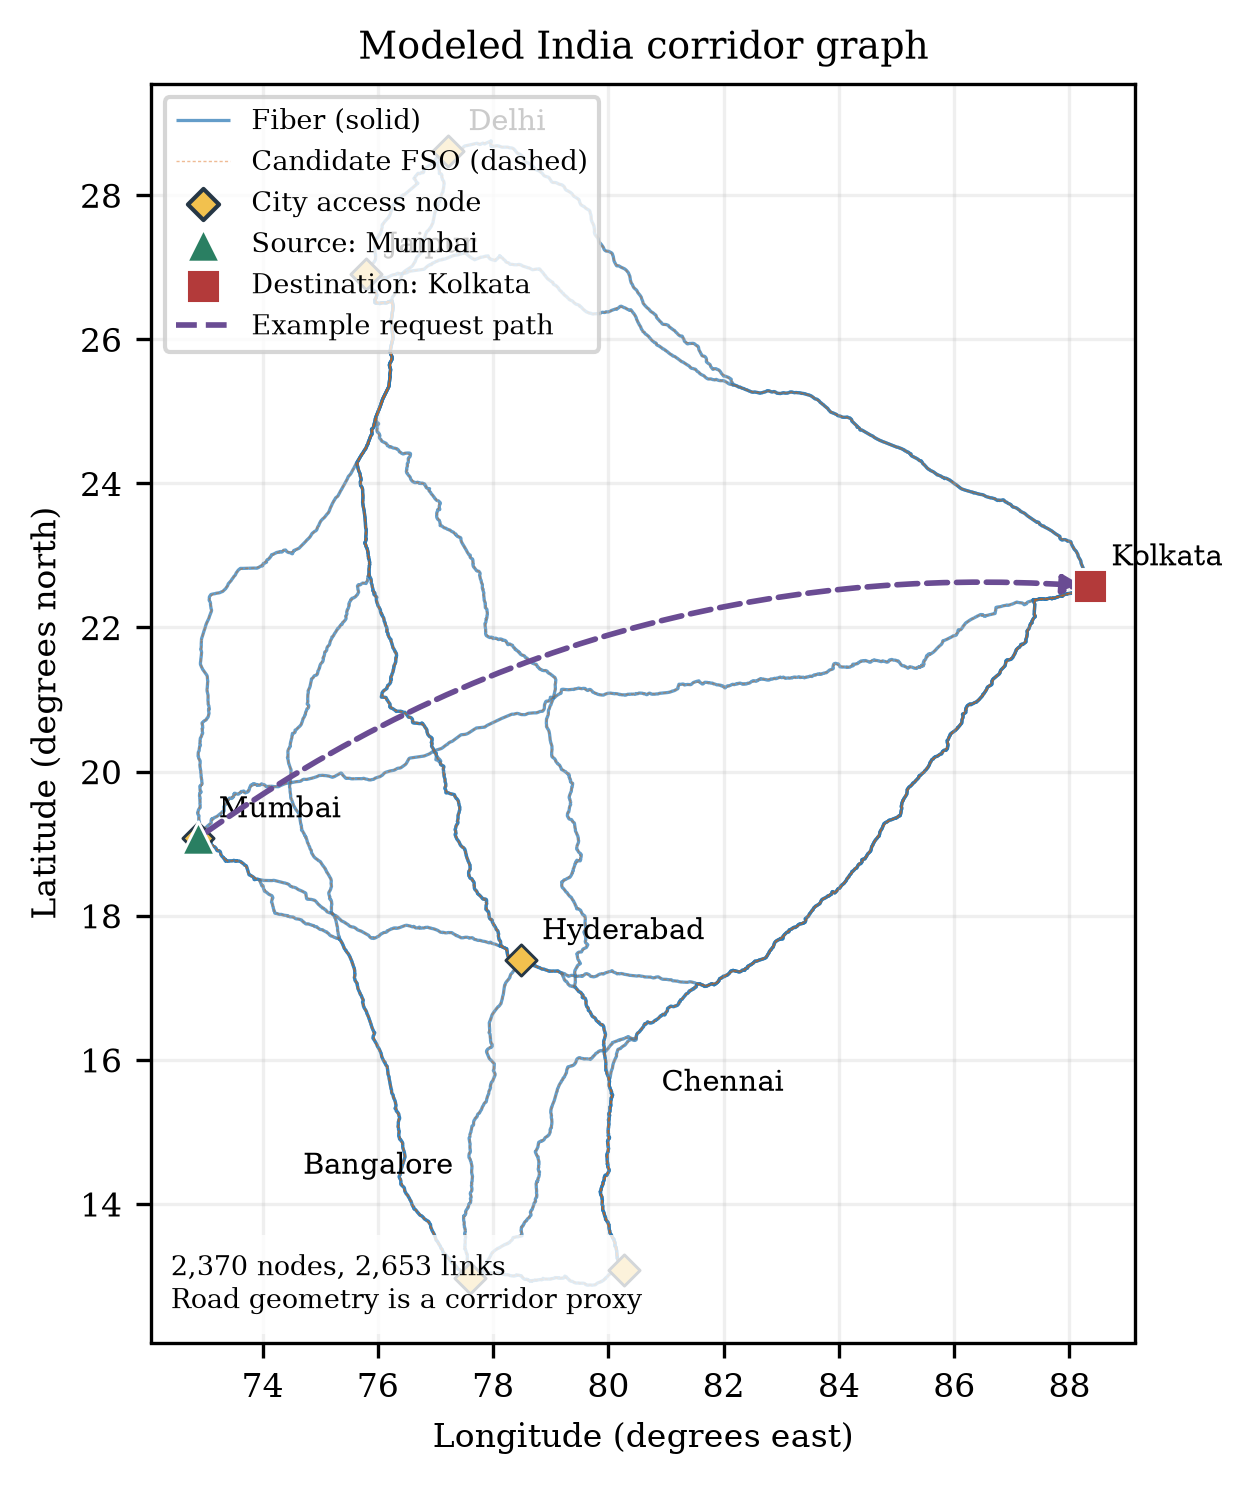
\includegraphics[width=0.78\linewidth]{corridor_map.png}
\caption{Modeled corridor graph. Solid blue lines show fiber, dashed orange lines show candidate FSO links, and symbols identify city access nodes and example request endpoints. The highlighted route is an example, not a verified physical path.}
\label{fig:topology}
\end{figure}

\section{Link and Scenario Models}
The fiber configuration uses a 1550-nm wavelength, an attenuation setting of 0.20~dB/km, detector efficiency of 0.93, and a measured dark-count upper bound below 70~s$^{-1}$. The FSO scenario uses a separate assumed 785-nm configuration, detector efficiency 0.60, dark counts of 100~s$^{-1}$, and an uncalibrated temporal correlation value of 0.85. The two configurations are not one characterized commercial terminal pair.

\begin{table}[htbp]
\centering
\caption{Representative link-model settings and their evidence class}
\label{tab:link-settings}
\begin{tabular}{@{}p{1.5in}p{0.9in}p{3.4in}@{}}
\toprule
Quantity & Setting & Evidence class \\
\midrule
Fiber wavelength & 1550 nm & Device profile \\
Fiber attenuation & 0.20 dB/km & Inherited target \\
Fiber detector efficiency & 0.93 & Reported device value \\
Fiber dark-count bound & $<70$ s$^{-1}$ & Reported upper bound \\
FSO wavelength & 785 nm & Scenario assumption \\
FSO detector efficiency & 0.60 & Scenario assumption \\
FSO dark counts & 100 s$^{-1}$ & Scenario assumption \\
FSO temporal correlation & 0.85 & Uncalibrated assumption \\
\bottomrule
\end{tabular}
\end{table}

The FSO channel includes atmospheric, diffraction, pointing, and background terms and uses a correlated log-normal turbulence process. Scenario labels represent normal, summer, and winter conditions at 02:00 and 22:00. These are synthetic scenario settings, not calibrated Indian meteorological traces.

\section{Matched Policy Architectures}
Both policies receive the same observation and use the same candidate-scoring interface, critic, feasibility rule, PPO loss, and training budget. The GNN encoder aggregates node and edge information through graph message passing. The LSTM encoder reads node-feature rows in a stable topology order and does not receive the graph edge index. Its recurrent state is initialized afresh for each policy call. Thus it is an ordered-node sequence encoder, not persistent temporal memory over route decisions. Figure~\ref{fig:architecture} distinguishes the shared and encoder-specific components.

\begin{figure}[htbp]
\centering
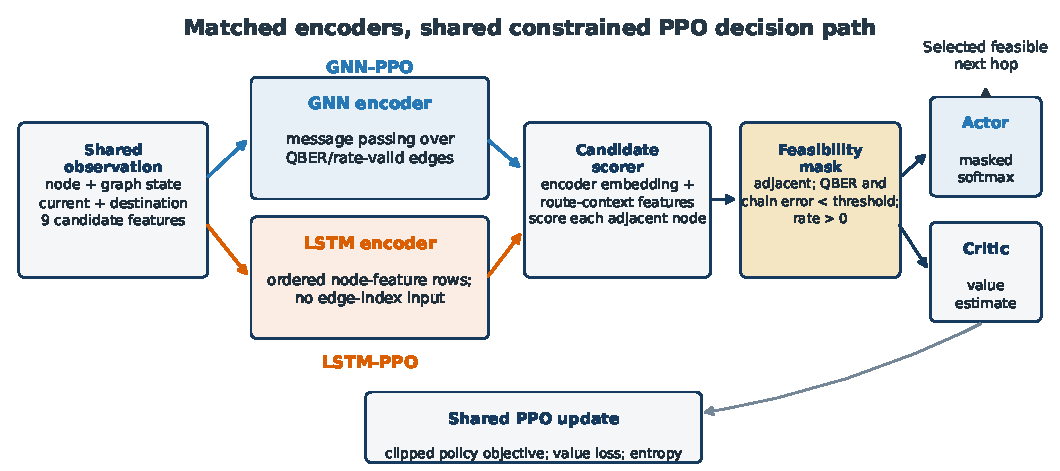
\includegraphics[width=0.95\linewidth]{matched_architecture.pdf}
\caption{Matched GNN-PPO and LSTM-PPO architecture. The policies share observations, candidate scoring, feasibility masking, actor--critic heads, and PPO updates; their encoders differ in graph message passing versus fixed-order node-sequence processing.}
\label{fig:architecture}
\end{figure}

\subsection{GNN-PPO Encoder}
The GNN maps node features into embeddings and updates them by neighborhood aggregation over valid graph edges. The actor combines the current-node, destination, and candidate-neighbor embeddings with candidate route-context features to produce action logits. Invalid full-graph edges are excluded from message passing under the configured link screen, and the candidate action mask additionally checks projected segment error.

\subsection{LSTM-PPO Encoder}
For node row $x_i$ at sequence position $i$, the LSTM computes
\begin{equation}
(h_i,c_i)=\operatorname{LSTM}(x_i,h_{i-1},c_{i-1}),\qquad h_0=c_0=0.
\label{eq:lstm}
\end{equation}
The resulting node representations feed the shared candidate scorer. The fixed order means that permuting node rows can alter the sequence neighborhoods even when the underlying graph is unchanged. This is an explicit architectural difference and a limitation of the comparator.

\subsection{Feasibility-Masked Policy}
The actor produces a logit $z_{v_t,u}$ for each adjacent candidate. Its probability is normalized only across the feasible actions:
\begin{equation}
\pi_\theta(u\mid o_t)=
\frac{\exp(z_{v_t,u})}
{\sum_{w\in\mathcal{A}_{\mathrm{feasible}}(s_t)}\exp(z_{v_t,w})},
\qquad u\in\mathcal{A}_{\mathrm{feasible}}(s_t).
\label{eq:policy}
\end{equation}
If the feasible set is empty, the episode terminates as a no-valid-action failure. The mask therefore defines the allowed choices, while the learned policy ranks candidates that remain.

\section{PPO Training}
PPO updates the policy using the clipped surrogate objective \cite{schulman2017},
\begin{align}
L^{\mathrm{clip}}(\theta)
=\mathbb{E}_t\Bigl[\min\bigl(&\rho_t(\theta)\hat A_t,\nonumber\\
&\operatorname{clip}(\rho_t(\theta),1-\epsilon,1+\epsilon)\hat A_t\bigr)\Bigr],
\label{eq:ppo}
\end{align}
where $\rho_t(\theta)=\pi_\theta(a_t\mid o_t)/\pi_{\theta_{\mathrm{old}}}(a_t\mid o_t)$ is the new-to-old action-probability ratio and $\hat A_t$ is the estimated advantage. The implementation also uses a value loss and entropy regularization. Hyperparameters are supplied by versioned experiment configurations.

\section{Experimental Protocol}
Five independent seeds are used per architecture (20261002--20261006). Both policies use 15 epochs of behavior cloning and 50 PPO epochs, with 144 steps per epoch. Test endpoint pairs and their reversals are excluded from demonstrations. PPO training uses Delhi to Chennai under the monsoon scenario at 22:00. Checkpoint selection uses a fixed monsoon validation suite; held-out scenarios remain reserved for final reporting.

\begin{table}[htbp]
\centering
\caption{Frozen matched training and held-out evaluation protocol}
\label{tab:protocol}
\small
\begin{tabular}{@{}p{1.8in}p{4.2in}@{}}
\toprule
Setting & Value \\
\midrule
Architectures & GNN-PPO and LSTM-PPO \\
Training seeds & 20261002, 20261003, 20261004, 20261005, 20261006 per architecture \\
Training budget & 15 BC epochs; 50 PPO epochs; 144 steps per PPO epoch \\
Training pair & Delhi--Chennai; monsoon; 22:00 \\
Validation & Delhi--Chennai; monsoon; seeds 11001--11004 \\
Held-out endpoints & Six ordered city pairs; reversals excluded from BC \\
Held-out conditions & Normal, summer, and winter, each at 02:00 and 22:00 \\
Replicates & Three shared environment replicates per pair/condition \\
Episodes & 108 per checkpoint; 540 per architecture \\
Episode limits & QBER threshold 0.11; fiber outage probability 0.01; 144 steps \\
\bottomrule
\end{tabular}
\end{table}

The held-out environment seeds are paired between architectures. Uncertainty intervals use a nested bootstrap: checkpoints are resampled outside, and shared scenario clusters are resampled within selected checkpoints. The primary effect is LSTM-PPO completion minus GNN-PPO completion on matched scenario identifiers.

\section{Evaluation Metrics}
Route completion is the primary endpoint and is defined by reaching the requested destination before modeled failure or truncation. Secondary reporting includes successful-route hop count, invalid actions, environment fallbacks, no-valid-action states, condition-level completion, and checkpoint variation. Hop count is conditional on success; it is not an efficiency measure for failed episodes.

Inference time is measured for deterministic actor calls on one CPU host after 100 warm-up calls, using 1,000 calls per checkpoint, four Torch threads, and disabled encoder caching. The measurement excludes environment simulation and deployment overhead. The LSTM evaluation used exact-input rollout memoization for repeated encoder computation; this changes computation time but not the policy output on an unchanged input. Encoder caching is disabled for the latency benchmark.

\chapter{Results}

\section{Matched Held-Out Comparison}
The final evaluation includes five frozen checkpoints per architecture and 108 paired scenarios per checkpoint, for 540 episodes per policy. GNN-PPO completed 249 routes (46.1\%; nested 95\% interval 31.3--58.5\%). LSTM-PPO completed 403 routes (74.6\%; 58.0--87.6\%). The paired LSTM-minus-GNN difference is 28.5 percentage points (nested 95\% interval 20.6--37.2).

Across the 540 matched outcomes, both policies succeeded on 242 scenarios, LSTM-PPO alone succeeded on 161, GNN-PPO alone succeeded on 7, and both failed on 130. Neither policy proposed invalid actions or used an environment fallback. GNN-PPO reached 18 no-valid-action states, while LSTM-PPO reached none. The shared failures show that the aggregate completion advantage does not mean that the task was broadly solved.

Figure~\ref{fig:primary} summarizes completion, the paired effect, and successful-route hops. Averaged checkpoint-specific successful-hop means were 87.8 for GNN-PPO and 71.4 for LSTM-PPO. Among the 242 scenarios completed by both policies, LSTM-PPO used 32.6 fewer hops on average.

\begin{figure}[htbp]
\centering
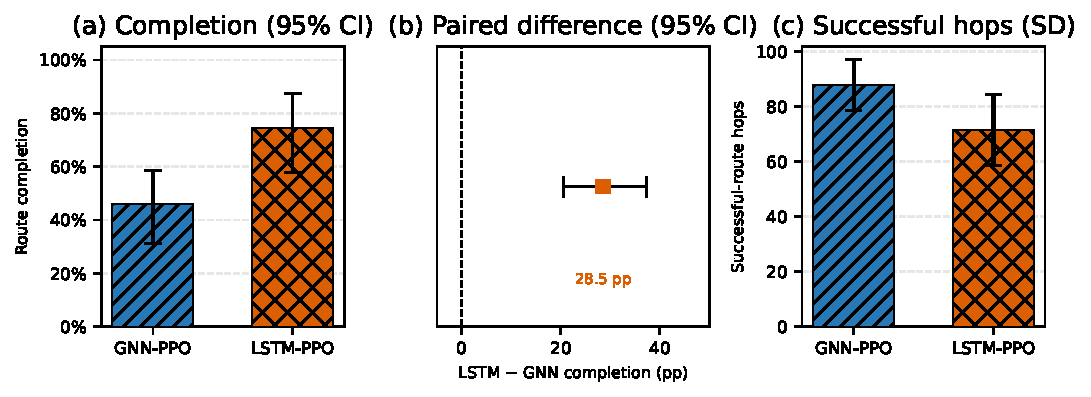
\includegraphics[width=0.96\linewidth]{01_gnn_lstm_primary.pdf}
\caption{Held-out GNN-PPO and LSTM-PPO comparison: route completion and its nested 95\% interval, the paired completion difference, and successful-route hops summarized across checkpoint means.}
\label{fig:primary}
\end{figure}

\section{Performance Across Conditions}
LSTM-PPO's mean completion exceeded GNN-PPO's in each of the six season/time conditions, with differences between 24.4 and 32.2 percentage points. These condition summaries show that the aggregate difference was not isolated to one cell. The number of independent checkpoints remains five per policy, so the condition patterns should be read with that seed sample in mind. Figure~\ref{fig:conditions} gives the condition-specific results.

\begin{figure}[htbp]
\centering
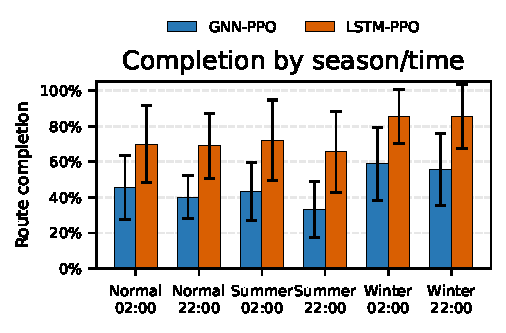
\includegraphics[width=0.9\linewidth]{02_gnn_lstm_by_condition.pdf}
\caption{Held-out completion across season and time conditions. Bars show means across five checkpoints; whiskers show checkpoint standard deviation.}
\label{fig:conditions}
\end{figure}

\section{Training-Seed Variation}
GNN-PPO checkpoint completion ranged from 18.5\% to 63.9\%; LSTM-PPO ranged from 42.6\% to 89.8\%. Figure~\ref{fig:seeds} shows the five matched checkpoint pairs. The training checkpoints, rather than the 540 scenario evaluations, are the replication units for training variation.

\begin{figure}[htbp]
\centering
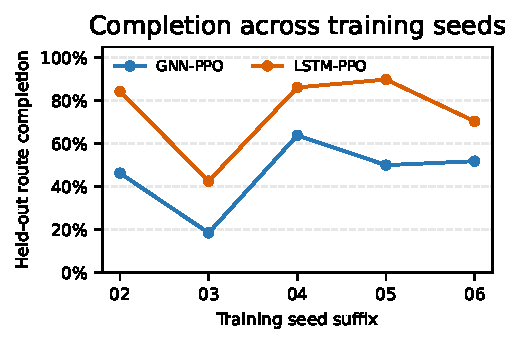
\includegraphics[width=0.86\linewidth]{03_gnn_lstm_seed_variability.pdf}
\caption{Held-out completion for each matched training-seed pair. Seed suffixes identify the five independently trained checkpoints.}
\label{fig:seeds}
\end{figure}

\section{Inference Cost}
The measured mean checkpoint-specific p95 actor-call latency was $9.61\pm1.65$~ms for GNN-PPO and $6.24\pm0.22$~ms for LSTM-PPO. These are checkpoint means and across-checkpoint standard deviations, obtained on the same CPU host after warm-up. They exclude environment simulation and do not measure end-to-end service latency. Figure~\ref{fig:latency} shows the measured comparison.

\begin{figure}[htbp]
\centering
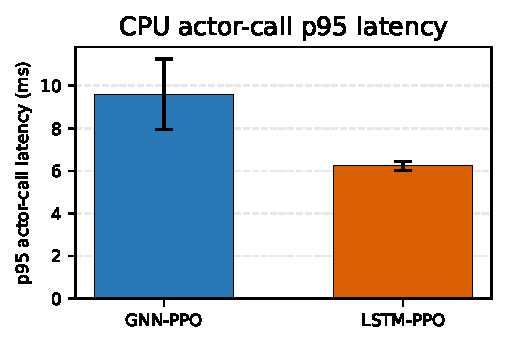
\includegraphics[width=0.78\linewidth]{04_gnn_lstm_latency.pdf}
\caption{CPU actor-call p95 latency in milliseconds, summarized across five checkpoints. Each checkpoint used 1,000 calls after warm-up, four CPU threads, and disabled encoder caching.}
\label{fig:latency}
\end{figure}

\section{Reward-Component Audit}
A separate diagnostic compares the 20261002 GNN-PPO and LSTM-PPO checkpoints on the same 108 scenario identifiers. GNN-PPO completed 50/108 routes (46.3\%) with 92.56 mean successful-route hops; LSTM-PPO completed 91/108 (84.3\%) with 62.22 hops. This selected-checkpoint result is descriptive and is not a second independent estimate of the five-seed comparison.

Figure~\ref{fig:reward} shows the component-wise cumulative reward difference. Components accumulate over trajectories of different lengths, so they describe the shaped training signal and are not independent measures of delivered key service. The figure is a reward audit, not an additional performance objective.

\begin{figure}[!tbp]
\centering
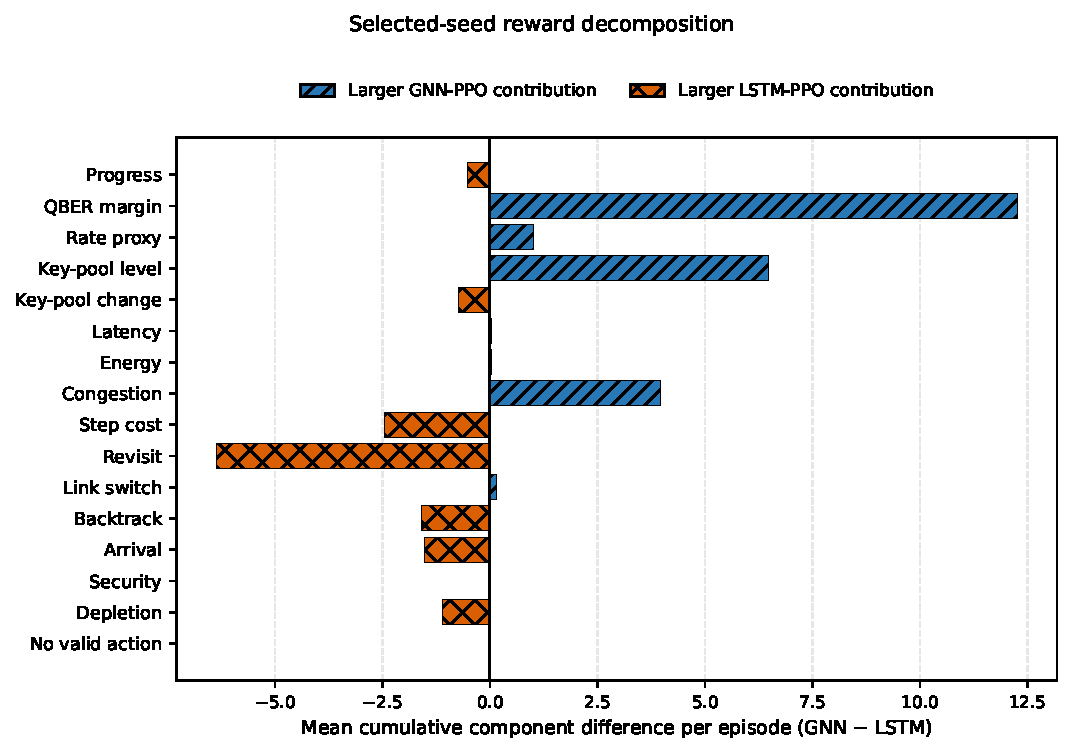
\includegraphics[width=0.96\linewidth]{05_gnn_lstm_reward_components.pdf}
\caption{Mean cumulative reward-component difference for selected matched checkpoints (GNN-PPO minus LSTM-PPO) on shared scenarios. The values are descriptive shaped-reward contributions; episode lengths differ.}
\label{fig:reward}
\end{figure}

\clearpage
\section{Model and Policy Diagnostics}
Analytical checks of the implemented fiber equations at 80~km and 1550~nm give modeled loss including excess loss of 16.46~dB, detection probability near 0.021 per incident photon, QBER proxy 0.0105, and normalized rate proxy 0.0175. For a 10-km FSO span in the monsoon 22:00 scenario, configured availability is 88\%; a 1,000-sample check produced 88.5\%, and the median normalized rate proxy conditional on availability was 0.2035. These are model checks, not device or field measurements.

Controlled paired-input counterfactuals on a selected GNN-PPO checkpoint held route context fixed while varying one candidate feature. FSO action probability rose from 0.311 to 0.638 as the normalized rate-proxy ratio to fiber rose from 0.25 to 4.0. With QBER below the feasibility threshold, action probability changed slightly from approximately 0.473 to 0.472; at QBER 0.111 the candidate was masked. In a separate 32-trial turbulence-input sweep, increasing the $C_n^2$ multiplier by a factor of 100 reduced median FSO rate proxy from 0.202 to 0.183. Mean FSO action probability moved from 0.749 to 0.740, and FSO remained selected in all trials. These are local policy-sensitivity diagnostics and do not establish route-level benefits or calibrated atmospheric response.

\chapter{Discussion}

\section{Interpretation of the Matched Comparison}
In the tested scenario matrix, LSTM-PPO achieved higher route completion, fewer conditional successful-route hops, and lower measured actor-call latency. The shared observation, PPO objective, training budget, candidate features, feasibility mask, and downstream decision interface make this a matched comparison of the implemented encoder-policy combinations. They do not make the encoders equivalent in capacity, inductive bias, or optimization behavior.

\section{Node-Order Sensitivity}
The LSTM processes rows in a fixed node order and does not receive the graph edge index. Its representation can therefore change when node rows are permuted, even if the graph itself is unchanged. The recurrent state is reset on every policy call and does not carry route history across decisions. The GNN, by contrast, aggregates over graph connectivity. No node-permutation, parameter-matched, graph-aware sequence, or persistent-memory ablation was conducted. The observed outcome must therefore be attributed to these implementations and this training procedure, not to an intrinsic ranking of LSTM and GNN architecture families.

\section{Training-Seed Variability}
Five checkpoints per architecture provide limited seed evidence. Nested intervals resample checkpoints and shared scenarios but cannot resolve run-to-run tails; broader claims need more seeds.

\section{Need for Classical Resource-Aware Comparators}
The matched study does not establish an advantage over strong classical routing algorithms. A hop-count BFS or static shortest path optimizes a different objective and does not automatically represent changing availability, feasibility, or key-pool state. A meaningful classical comparator should use the same topology, route termination rules, feasibility checks, dynamic resource state, and held-out scenarios, with a defined resource-aware cost or state-dependent replanning rule. Such a baseline remains outside this evaluation.

\section{Limitations}
The corridor geometry is an OpenStreetMap road proxy, not verified fiber infrastructure. FSO line of sight, terrain clearance, and seasonal weather are not surveyed or calibrated. The fiber and FSO settings do not represent one characterized terminal pair. The key-pool state is normalized and single-route; calibrated generation and consumption, simultaneous demand, network-wide blocking, and management traffic are not modeled. The rate proxy is not delivered secret-key throughput, and the optional finite-key estimator is not independently established as composably secure. Inference timing is a single-host actor-call measurement rather than an end-to-end deployment result.

The exact reward-oracle check uses a static toy graph and a different state/action setting. It is retained as a separate diagnostic and is not pooled with the matched encoder evaluation. The current report also does not generalize beyond the tested architecture, topology, simulator assumptions, training budget, and held-out scenario distribution.

\chapter{Conclusion and Future Work}
This report presents a matched simulator study of GNN-PPO and LSTM-PPO for constrained next-hop routing in a modeled hybrid fiber/FSO trusted-node network. In the five-seed held-out evaluation, LSTM-PPO completed 74.6\% of routes compared with 46.1\% for GNN-PPO, a paired difference of 28.5 percentage points (nested 95\% interval: 20.6--37.2). The result supports the tested ordered-node LSTM implementation on this scenario matrix; it does not establish a general architecture ranking or field performance.

Further work should measure node-permutation sensitivity, test parameter-matched and graph-aware sequence encoders, include persistent recurrent state as a separate baseline, and increase the number of independent training seeds. It should also evaluate resource-aware classical routing under the same dynamic feasibility rules, test broader topologies and traffic settings, and calibrate channel and key-pool models against traceable measurements before drawing service or deployment conclusions.

\section*{Data and Code Availability}
\addcontentsline{toc}{chapter}{Data and Code Availability}
The project repository contains the simulator, experiment configurations, evaluation outputs, figure-generation scripts, and manuscript sources. Corridor geometry is based on OpenStreetMap data and must be credited under its applicable terms. The geometries are routing proxies and do not represent verified fiber infrastructure.

\appendix
\chapter{Reproducibility Summary}
The matched study uses five independently trained seeds per architecture, identical 15-epoch BC and 50-epoch PPO budgets, validation-only checkpoint selection, and paired held-out scenario identifiers. The complete protocol and resolved configurations are retained with the project artifacts. The final test set contains six ordered city pairs, six season/time conditions, and three environment replicates per checkpoint.

The primary figure reports route completion and its nested interval. Companion figures report condition-level completion, checkpoint variation, actor-call latency, and the separate reward-component audit. The selected-checkpoint reward audit and small-graph oracle check are kept separate from the five-seed matched encoder estimate.

\bibliographystyle{IEEEtran}
{\small
\setlength{\parskip}{0pt}
\bibliography{../paper/references}
}

\end{document}
